%https://tex.stackexchange.com/questions/139686/controlling-orientation-in-3d-pgf-plots

\documentclass[border=2pt, tikz]{standalone}
\usepackage{pgfplots}
\pgfplotsset{compat=1.16}
\usetikzlibrary{calc}

\begin{document}

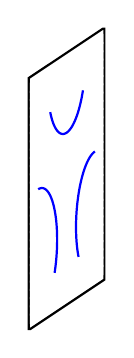
\begin{tikzpicture}

\begin{axis}%
[ scale=0.8
, hide axis
%, axis lines=middle, axis on top
, x={(-0.3cm,-0.2cm)}, y={(1.5cm,0.0cm)}, z={(0cm,1cm)}
%, view={115}{30} % {rotation angle}{elevation angle}
%, xlabel=$x$
%, ylabel=$y$
%, zlabel=$z$
, zmin=-2
, zmax=2
, xmin=-2
, xmax=2
, ymin=-2
, ymax=2
, declare function={
        s(\t) = (\t+30)/90;
    }
]

%% Parabola and cubic shadow curves
%\addplot3%
%[ samples=40
%, samples y=0
%, thick 
%, cyan 
%, domain=-2:2
%, variable=\t
%] ({t},{t^2},{-8});
%
%\addplot3%
%[ samples=40
%, samples y=0
%, thick
%, red 
%, domain=-2:2
%, variable=\t
%] ({t},{-1},{t^3});

%  Lines
%  (pgfplots cannot handle a \foreach commands inside the {axis} environment, so the draw commands need to have the foreach inside of them. See also pgfplotsinvokeforeach._

%\draw [cyan] foreach \a in {-2,-1.9,...,2} {
%({\a}, {(\a)^2}, {(\a)^3}) --  ({\a}, {(\a)^2}, -8)
%};
%



\draw [black, thick]  {
(-2,0,-2) -- (2, 0, -2) -- (2,0,2) -- (-2,0,2) -- cycle
};
\addplot3[mesh,
	color=white,
	samples=30,
%	mesh/line width=1mm,
	line width=0.2mm,
%	faceted color=gray!40!white,
%	faceted color=none,
%	draw=none,
	opacity=0.9,
	domain=-1.9:1.9,    % x 范围
    y domain=-1.9:1.9,  % y 范围
    ] 
    (x,0,y);
%\addplot3[
%    fill=gray!20,
%    draw=black,
%    thick,
%]
%coordinates {
%(-2,0,-2)
%(2,0,-2)
%(2,0,2)
%(-2,0,2)
%(-2,0,-2)
%};

% Twisted cubic


\foreach \k in {0,1,2}
{


\addplot3%
[ samples=100
, samples y=0
, thick
, blue 
, domain=-60:60
, variable=\t
] 
({cos (t-90+120*\k)-sqrt(3)*sin(120*\k)},{0},{sin (t-90+120*\k)+sqrt(3)*cos(120*\k)});



}

\end{axis}
\end{tikzpicture}
\end{document}